\documentclass{article}
\usepackage{amsmath}
\usepackage{amssymb}
\usepackage{tikz}
\usetikzlibrary{calc}

\begin{document}

\title{Analysis of problem UVA 11692 --- Rain Fall}
\date{}
\author{Tiago Royer}
\maketitle

(To minimize subscripts,
I will use $R$ for $T_1$, the duration of the rainfall,
and $D$ for $T_2$, the delay between ending the rain and the observation.)

Let's call $f: \mathbb R \to \mathbb R$
the function that maps the time (in hours) since the beginning of the rain
and the height (in millimeters) in the tube.

Since the tube starts empty, $f(0) = 0$.
Then, the tube fills at an uniform, unknown rate $c$,
until it level reaches $L$
(the leak height),
at some time $t$.
Then, due to the leakage,
the filling rate is now $c - K$,
until the time reaches $R$ (when the rain ends).
Now, in the abscence of rain,
the level drops at rate $K$,
solely due to the leakage,
until the water level matches the leak at time $t'$;
finally, the level remains stable until the observation.

The graph of $f$ is shown in figure~\ref{fig1}.

\begin{figure}[h]
    \centering
    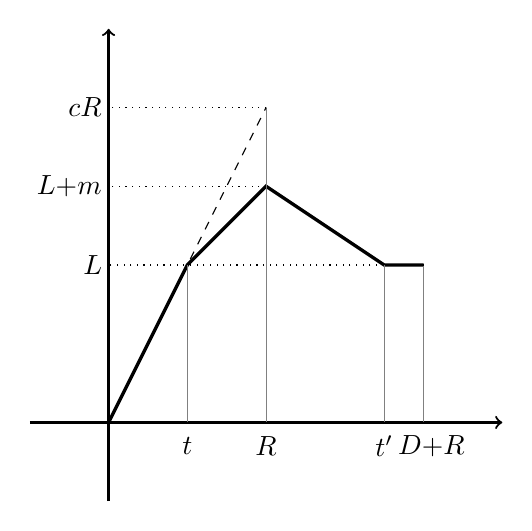
\begin{tikzpicture}
        \coordinate (L) at (1, 2); % Point where it reaches the leakage
        \coordinate (Lx) at (1, 0); % L in x-axis
        \coordinate (Ly) at (0, 2); % L in y-axis
        \coordinate (R) at (2, 3); % Point when the rain ends
        \coordinate (Rx) at (2, 0);
        \coordinate (Ry) at (0, 3);
        \coordinate (MR) at (2, 4); % Maximum possible rain value
        \coordinate (MRy) at (0, 4);
        \coordinate (D) at (3.5, 2); % How many water "drops" out of the tube
        \coordinate (Dx) at (3.5, 0);
        \coordinate (Dy) at (0, 2);
        \coordinate (O) at (4, 2); % Observation
        \coordinate (Ox) at (4, 0);
        \coordinate (Oy) at (0, 2);

        \draw[thick, ->] (-1, 0) -- (5, 0);
        \draw[thick, ->] (0, -1) -- (0, 5);

        \draw[very thick] (0, 0) -- (L) -- (R) -- (D) -- (O);

        \begin{scope}[gray,thin]
            \draw (L) -- (Lx);
            \draw (MR) -- (Rx);
            \draw (D) -- (Dx);
            \draw (O) -- (Ox);
        \end{scope}

        \begin{scope}[dotted, thin]
            \draw (O) -- (Oy);
            \draw (R) -- (Ry);
            \draw (MR) -- (MRy);
        \end{scope}

        \path (Lx) ++(0, -0.3) node {$t$};
        \path (Rx) ++(0, -0.3) node {$R$};
        \path (Dx) ++(0, -0.3) node {$t'$};
        \path (Ox) ++(0.1, -0.3) node {$D{+}R$};

        \draw[dashed] (0, 0) -- (MR);
        \path (MRy) ++ (-0.3, 0) node {$cR$};
        \path (Ly) ++ (-0.2, 0) node {$L$};
        \path (Ry) ++ (-0.5, 0) node {$L{+}m$};

    \end{tikzpicture}

    \caption{$f$'s graph.}
    \label{fig1}
\end{figure}

The dashed line represents how high the level of rain would be
if there were no leakage.
This is the actual amount of rain,
and the value the problem asks.
We must give both the smallest and the highest possible value of $cR$,
while still retaining the specified observation height.

If the leakage is above the observation height
--- that is, $L > H$ ---,
then there had no leakage,
so the amount of rain must be exactly $H$.
If the observation height is strictly above the leakage
--- $L < H$ ---,
the value $t'$ is actually after $D+R$ (see figure~\ref{fig2});
moreover,
the value $L+m$ (the maximum water level)
can be computed exactly.
Therefore, the amount of rain itself can be computed exactly;
thus, the minimum equals the maximum again.
And finally, if $L = H$,
the minimum possible amount of rain is exactly $L$,
since that's just enough so that the water level touches the leak
(in this case, $t = R = t'$),
and the maximum occours when the tube has just stopped leaking when we observe,
thus making the value $L+m$ as high as possible
(in this case, $t' = D+R$).

\begin{figure}[h]
    \centering
    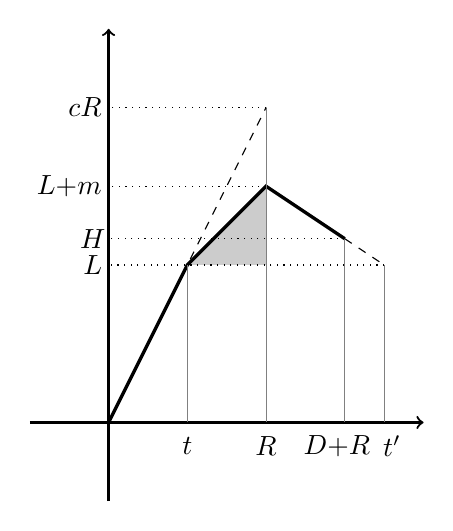
\begin{tikzpicture}
        \coordinate (L) at (1, 2);
        \coordinate (Lx) at (1, 0);
        \coordinate (Ly) at (0, 2);
        \coordinate (R) at (2, 3);
        \coordinate (Rx) at (2, 0);
        \coordinate (Ry) at (0, 3);
        \coordinate (MR) at (2, 4);
        \coordinate (MRy) at (0, 4);
        \coordinate (O) at (3, 2.3333); % Adjusted for when D = 1
        \coordinate (Ox) at (3, 0);
        \coordinate (Oy) at (0, 2.3333);
        \coordinate (D) at (3.5, 2); % Full delay
        \coordinate (Dx) at (3.5, 0);
        \coordinate (Dy) at (0, 2);

        % This triangle needs to appear below everything
        \fill[black!20] (L) -- (R) -- ($(Rx) + (Ly)$) -- cycle;

        \draw[thick, ->] (-1, 0) -- (4, 0);
        \draw[thick, ->] (0, -1) -- (0, 5);

        \draw[very thick] (0, 0) -- (L) -- (R) -- (O);

        \begin{scope}[gray,thin]
            \draw (L) -- (Lx);
            \draw (MR) -- (Rx);
            \draw (D) -- (Dx);
            \draw (O) -- (Ox);
        \end{scope}

        \begin{scope}[dotted, thin]
            \draw (O) -- (Oy);
            \draw (R) -- (Ry);
            \draw (MR) -- (MRy);
            \draw (D) -- (Dy);
        \end{scope}

        \path (Lx) ++(0, -0.3) node {$t$};
        \path (Rx) ++(0, -0.3) node {$R$};
        \path (Ox) ++(-0.1, -0.3) node {$D{+}R$};
        \path (Dx) ++(0.1, -0.3) node {$t'$};

        \draw[dashed] (0, 0) -- (MR);
        \draw[dashed] (O) -- (D);

        \path (MRy) ++ (-0.3, 0) node {$cR$};
        \path (Ly) ++ (-0.2, 0) node {$L$};
        \path (Ry) ++ (-0.5, 0) node {$L{+}m$};
        \path (Oy) ++(-0.2, 0) node {$H$};

    \end{tikzpicture}

    \caption{$f$'s graph, when $L < H$.}
    \label{fig2}
\end{figure}

We thus have already solved the problem when $L > H$,
and found the minimum when $L = H$.
If $L < H$, the maximum equals the minimum;
so, it remains to compute the maximum value when $L \leq H$.

First, let's express $t$ in terms of $c$.
We have $f(t) = L$.
As $f(x) = cx$ in $[0, l]$,
we have
\begin{equation*}
    f(t) = ct = L.
\end{equation*}
Thus,
\begin{equation*}
    t = \frac L c.
\end{equation*}
As the value $L$ is given by the problem,
this equation effectively express $t$ using only $c$.

Now, we will isolate $m$.
Due to the leakage, $f'(x) = -K$ for $x \in (R, D+R)$.
As $f(D+R) = H$ and $f$ is continuous,
this means that
\begin{align*}
    f(R+D) &= -KD + f(R) \\
    H &= -KD + f(R) \\
    f(R) &= H + KD \\
\intertext{Replacing $f(R)$ by $L + m$ gives}
    L + m &= H + KD \\
    m &= H + KD - L.
\end{align*}
Observe that these equations works both when $H = L$ and $H > L$.

Now, consider the triangle shaded in figure~\ref{fig2}.
Its height is exactly $m$,
and its base is $R - t$.
The slope of it's hypotenuse equals $f'(x)$ for $x \in (t, R)$;
by the reasoning above, this is $c - K$.
(Note we may assume $c > K$ since we are maximizing $c$.%
\footnote{
    If $c \leq K$, then $f$ would remain steady between $t$ and $R$,
    so there would not be any leakage between $R$ and $D+R$.
    This would happen if $D = 0$,
    leaving no time to happen any leakage;
    but the problem guarantees that every value is greater than $0.01$,
    leaving at least some seconds to leak
    and allowing us to assume $c > K$.
})
The slope of the hypothenuse is the ratio of the catheti;
thus,
\begin{align*}
    c - K &= \frac{m}{R - t}. \\
\intertext{Proceeding the computation,}
    (c - K)*(R - t) &= m \\
    cR - ct - KR + Kt &= m \\
    Rc - (L + KR + m) + \frac{KL}{c} &= 0 \\
    Rc - (H + KR + KD) + \frac{KL}{c} &= 0 \\
\intertext{Multiply everything by $c$ gives the quadratic equation}
    Rc^2 - (H + KR + KD)c + KL &= 0.
\end{align*}

Using the quadratic formula (with $a = R$, $b = -(H+KR+KD)$, $c = KL$):
\begin{align*}
    c &= \frac{-b \pm \sqrt{b^2 - 4ac}}{2a} \\
      &= \frac{H + KR + KD \pm \sqrt{(H+KR+KD)^2 - 4RKL}}{2R}
\end{align*}

Intuitively, we are maximizing $c$,
so the answer is given using the ``$+$'' branch of the equation.
Actually, chosing ``$-$'' contradicts the assumption $c > K$:
\begin{align*}
    c &> K \\
    \frac{H + KR + KD - \sqrt{(H+KR+KD)^2 - 4RKL}}{2R} &> K \\
    H + KR + KD - \sqrt{(H+KR+KD)^2 - 4RKL} &> 2RK \\
    H + KD - \sqrt{(H+KR+KD)^2 - 4RKL} &> RK \\
    H + KD - KR &> \sqrt{(H+KR+KD)^2 - 4RKL} \\
    (H + KD - KR)^2 &> (H+KR+KD)^2 - 4RKL \\
    \Big((H + KR + KD) - 2KR\Big)^2 &> (H+KR+KD)^2 - 4RKL \\
    (H + KR + KD)^2 - 4KR(H + KR + KD) + 4K^2R^2 &> (H+KR+KD)^2 - 4RKL \\
    -4KR(H + KR + KD) + 4K^2R^2 &> - 4RKL \\
    -4(H + KR + KD) + 4KR &> - 4L \\
    -4H -4KR -4KD + 4KR &> - 4L \\
    -4KD &> 4(H-L) \\
\end{align*}
Both $K$ and $D$ are positive, and thus $0 > -4KD$.
We are treating the case $H \geq L$;
thus, $4(H-L) \geq 0$,
and this equation degenerates to
\begin{equation*}
    0 > -4KD > 4(H-L) \geq 0,
\end{equation*}
clearly a contradiction.

Therefore, we must take the ``$+$'' branch of the quadratic formula:
\begin{equation*}
    c = \frac{H + KR + KD + \sqrt{(H+KR+KD)^2 - 4RKL}}{2R},
\end{equation*}
and the answer to the problem is
\begin{equation*}
    cR = \frac{H + KR + KD + \sqrt{(H+KR+KD)^2 - 4RKL}}{2}.
\end{equation*}
\hfill $\square$
\end{document}
